\documentclass[mathserif]{beamer}

\usepackage{lmodern}
\usepackage{graphicx}
\usepackage{wrapfig}
\usepackage[T2A]{fontenc}
\usepackage[utf8]{inputenc}
\usepackage[ukrainian]{babel}
\usepackage{afterpage}
\usepackage{placeins}
\usepackage{cmap}
\usepackage[labelsep=period]{caption}
\usepackage{subcaption}
\usepackage{hyperref}

\setbeamertemplate{navigation symbols}{}
\usetheme{Boadilla}
\usecolortheme{default}

\hypersetup{colorlinks=true,linkcolor=blue,urlcolor=blue,citecolor=blue,anchorcolor=blue}

\title{Universal Sentence Encoder}
\institute{prom.ua}
\author[Д.О.~Петраківський]{Данило Олександрович Петраківський \\ d.petrakivskyi@smartweb.com.ua}
\date{\today}
\logo{
\includegraphics[height=10mm]{images/prom}\hspace{7pt}}

\begin{document}
    \frame{\titlepage}

    \begin{frame}{Universal Sentence Encoder}
        \href{https://arxiv.org/abs/1803.11175}{Universal Sentence Encoder} --- алгоритм векторизації рядків тексту,
        зокрема речень, словосполучень та коротких абзаців.
    \end{frame}

    \begin{frame}{Семантична подібність речень}
        \begin{figure}[h!]
            \centering
            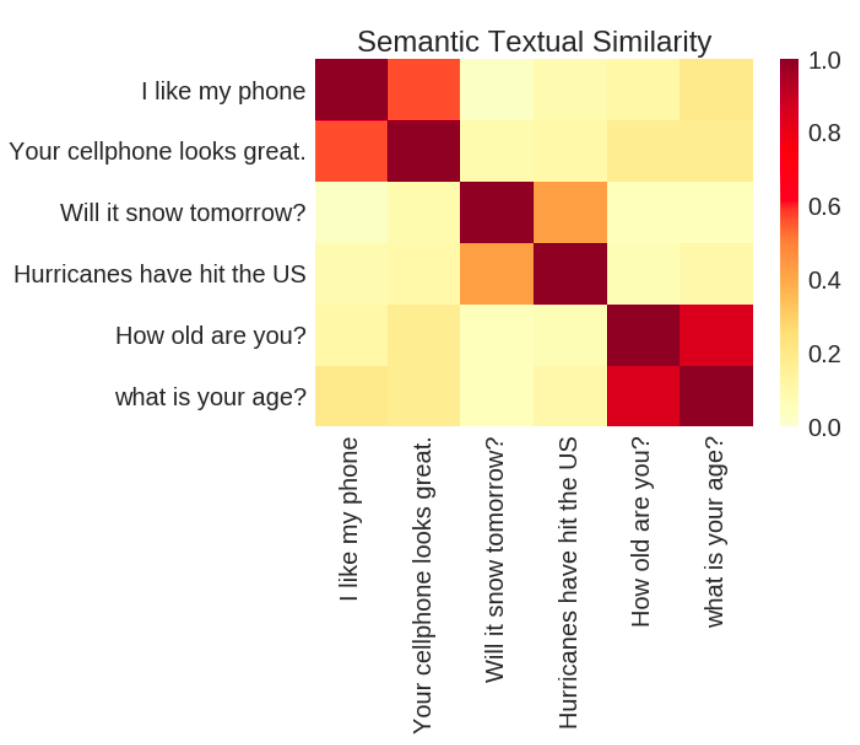
\includegraphics[width=200px]{images/use-sts}
        \end{figure}
    \end{frame}

    \begin{frame}{Приклад застосування}
        \begin{figure}[h!]
            \centering
            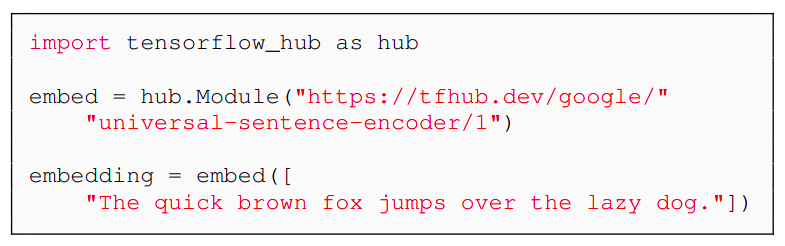
\includegraphics[width=250px]{images/use-code}
        \end{figure}
    \end{frame}

    \begin{frame}{Міра подібності речень}
        Для визначення схожості двох рядків слід застосувати наступну формулу до їхніх векторів $\boldsymbol{u}$ та
        $\boldsymbol{v}$:

        \[
            sim(\boldsymbol{u}, \boldsymbol{v})
            = 1
            - \arccos \biggl(\frac{\boldsymbol{u} \cdot \boldsymbol{v}}{||\boldsymbol{u}|| \ ||\boldsymbol{v}||}\biggr) / \pi.
        \]
    \end{frame}

    \begin{frame}
        \begin{center}
            \Huge \bfseries \itshape Дякую за увагу!
        \end{center}
    \end{frame}
\end{document}
